\documentclass[12pt]{article}

% Packages for math and formatting
\usepackage{amsmath}
\usepackage{amssymb}
\usepackage{amsthm}
\usepackage{mathrsfs}
\usepackage{fancyhdr}
\usepackage{graphicx}
\usepackage{subcaption}
\usepackage{setspace}
\usepackage{listings}
% \usepackage{xcolor}

\usepackage{newtxtext}
\usepackage{lipsum}
\usepackage[strict]{changepage}
\usepackage{framed}
\usepackage{float}
\usepackage[letterpaper,left=1in,right=1in,top=1in,bottom=1in]{geometry}
% \usepackage{tcolorbox}
\usepackage{cite}
\usepackage{bm}
% \usepackage[colorlinks,linkcolor=Black,filecolor=Black,urlcolor=RoyalBlue,citecolor=Cyan,bookmarks=true,bookmarksopen=false,pdfpagemode=FullScreen,pdfstartview=Fit]{hyperref}
\usepackage[dvipsnames,svgnames]{xcolor}
% \usepackage{tcolorbox}
% \definecolor{Brown}{RGB}{139,69,19} 
\usepackage[colorlinks,linkcolor=Brown,filecolor=Black,urlcolor=RoyalBlue,citecolor=Brown,bookmarks=true,bookmarksopen=false,pdfpagemode=FullScreen,pdfstartview=Fit]{hyperref}
\usepackage{indentfirst}
\usepackage{multicol}
\usepackage[square,numbers,sort&compress]{natbib}
% \usepackage{refcheck} % To output uncited references

\linespread{1.0}% Set line spacing to single
\renewcommand{\baselinestretch}{1}% Set single line spacing
\setlength{\parindent}{1.5em}% Set paragraph indentation
\setlength{\parskip}{0em}% Remove paragraph spacing
\raggedbottom% Avoid stretching pages

\newcommand{\R}{\mathbb{R}}
\newcommand{\F}{\mathbb{F}}
\newcommand{\N}{\mathbb{N}}
\newcommand{\Q}{\mathbb{Q}}
\newcommand{\Z}{\mathbb{Z}}
\newcommand{\0}{\boldsymbol{0}}
\newcommand{\setparDis}{\setlength{\parskip}{0.3cm}}
% \tcbuselibrary{most}

\setlength{\parskip}{0em}% Set paragraph spacing to 0, keep single line spacing
\setlength{\parindent}{1.5em}% Set paragraph indentation
\renewcommand{\baselinestretch}{1}% Set single line spacing
\renewcommand{\familydefault}{\rmdefault}% Set default font to Times New Roman
\usepackage{microtype}% Ensure full justification

\lstset{ %
    language=Matlab,                % 语言选择
    basicstyle=\ttfamily\small,     % 字体样式和大小
    keywordstyle=\color{blue},      % 关键字的颜色
    commentstyle=\color{gray},      % 注释的颜色
    stringstyle=\color{red},        % 字符串的颜色
    numbers=left,                   % 行号位置 (左侧)
    numberstyle=\tiny\color{gray},  % 行号的样式
    stepnumber=1,                   % 行号增量
    numbersep=5pt,                  % 行号与代码的距离
    backgroundcolor=\color{white},  % 背景色
    showspaces=false,               % 不显示空格符
    showstringspaces=false,         % 不显示字符串中的空格符
    showtabs=false,                 % 不显示制表符
    frame=single,                   % 给代码加上边框
    tabsize=4,                      % 设置制表符宽度
    captionpos=b,                   % 标题位置
    breaklines=true,                % 自动换行
    breakatwhitespace=true,         % 只在空格处换行
    title=\lstname,                 % 显示代码名称
    escapeinside={\%*}{*)},         % 在代码中加入LaTeX指令
    morekeywords={*,...}            % 自定义更多关键词
}

\setstretch{1.2}
\setlength{\parskip}{1em}

% Geometry settings for better margins
% \geometry{a4paper, margin=1in}

% Header and footer
\pagestyle{fancy}
\fancyhf{}
\fancyhead[L]{Kecai Xuan}
\fancyhead[C]{Math Homework}
\fancyhead[R]{\today}
\fancyfoot[C]{\thepage}

\begin{document}

\setlength{\parindent}{0pt}

\begin{titlepage}
    \centering

    %------------------------------------------------------------
    %    Top rules
    %------------------------------------------------------------

    \rule{\textwidth}{1pt}   % The top horizontal rule
    \vspace{0.04\textheight}  % Whitespace between top horizontal rule and title

    %------------------------------------------------------------
    %    Title
    %------------------------------------------------------------

    \begin{figure}[ht]
      \centering
      
\includegraphics[width=0.4\textwidth]{../img/University_of_Maryland_seal.png}
    \end{figure}

    \vspace{0.07\textheight}
        {\Huge \textbf{AMSC660 Final Report}}  % Title

    
    \vspace{0.03\textheight}

    % \vspace{0.02\textheight}   % Whitespace between the title and short horizontal rule

    \rule{0.83\textwidth}{0.4pt}  % The short horizontal rule under title

    \vspace{0.04\textheight}  % Whitespace between the short horizontal rule and author

    %------------------------------------------------------------
    %    Author
    %------------------------------------------------------------

    {\large \textsc{Department of Chemistry and Biochemistry, University of Maryland}}

    \vspace{0.013\textheight}

    {\large \textsc{Kecai Xuan}}

    \vspace{0.013\textheight}

    {\large \href{https://github.com/Bessgendre/AMSC660-Final-2024}{https://github.com/Bessgendre/AMSC660-Final-2024}}

    \vspace{0.013\textheight}

    \vspace{0.04\textheight}

    % {\Large \textsc{}}

    \vfill  % Whitespace between author and date

    {\large \today}  % The date at the bottom of the page
    \vspace{0.04\textheight}  % Whitespace between date and bottom horizontal rule

    %------------------------------------------------------------
    %    Bottom rules
    %------------------------------------------------------------

    \rule{\textwidth}{1pt}  % The bottom horizontal rule

\end{titlepage}

\section{Linear Discriminant Analysis}

\subsection{Rank of $\mathbf{S_b}$}

Consider the vector set $\{m_1 - m, m_2 - m,\cdots m_c-m\}$, we have the following relation:
\[
    \sum_{i=1}^c n_i\left(m_i-m\right)=\bigg[\sum_{i=1}^c n_i m_i\bigg]-n m=n m-n m=0
\]
which means that there exist the nonzero linear combination parameters such that the sum of the vectors is zero. Therefore, the vector set is linearly dependent.

Since $S_b$ is defined as
\[
    \displaystyle S_b=\sum_{i=1}^c n_i\left(m_i-m\right)\left(m_i-m\right)^\top
\]
a weighted sum of these rank-1 matrices, it follows that the image (or output) of the linear transformation defined by $S_b$ lies within the space spanned by the vector set $\{m_1 - m, m_2 - m,\cdots m_c-m\}$. That is because when applying $S_b$ to any vector $x$, it gives the linear combination of the vectors in the set:
\[
    S_b x = \sum_{i=1}^c n_i\left(m_i-m\right)\left(m_i-m\right)^\top x
\]
where $\left(m_i-m\right)^\top x$ is a scalar. 

The rank of matrix $S_b$ is equal to the dimension of its image, which is the space spanned by the vector set $\{m_1 - m, m_2 - m,\cdots m_c-m\}$ that is linearly dependent. Therefore, the rank of $S_b$ is at most $c-1$.

\subsection{Gradient of $\mathbf{J(w)}$}

The gradient of $J(w)$ is given by
\begin{align*}
    \nabla J(w) &= \nabla \left(\frac{w^\top S_b w}{w^\top S_w w}\right)\\
    &= \frac{2}{(w^\top S_w w)^2} \bigg[ (w^\top S_w w) S_b w - (w^\top S_b w) S_w w \bigg]
\end{align*}
Let it be zero, we have $(w^\top S_w w) S_b w - (w^\top S_b w) S_w w = 0$, where $w^\top S_w w, w^\top S_b w$ are scalars. So the only way to get the equation satisfied is to have 
\[
    S_b w = \lambda S_w w, \quad \lambda = \frac{w^\top S_b w}{w^\top S_w w}
\]

\subsection{Cholesky Decomposition}

It is obvious that $S_w$ is a SPD matrix, which can be decomposed as $S_w = L L^\top$. Define $y = L^\top w, w = L^{-\top} y$, then the equation $S_b w = \lambda S_w w$ can be rewritten as
\begin{align*}
    S_b L^{-\top} y = \lambda L y \quad \Rightarrow \quad  L^{-1} S_b L^{-\top} y = \lambda y
\end{align*}
which takes the form of $Ay = \lambda y$ where $A = L^{-1} S_b L^{-\top}$ is SPD.
    
\subsection{LDA Performance and Comparison with PCA on MINST}

The projection of the data onto the first two linear discriminants and the first two principal components are shown in the following figure. For this problem, tt is clear that the linear discriminants are able to separate the data better than the principal components.

\begin{figure}[h!]
    \centering
    % Subfigure for LDA
    \begin{subfigure}[b]{0.45\textwidth}
        \centering
        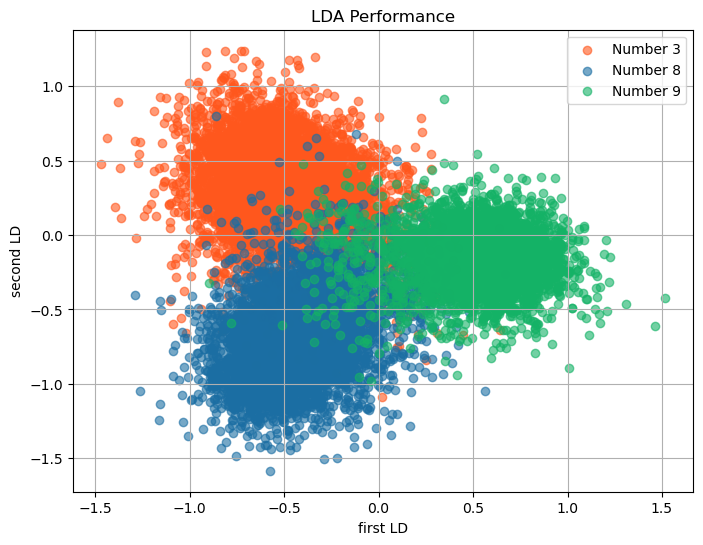
\includegraphics[width=\textwidth]{../img/problem_1/LDA.png}
        \caption{LDA Performance}
        \label{fig:lda}
    \end{subfigure}
    \hfill
    % Subfigure for PCA
    \begin{subfigure}[b]{0.45\textwidth}
        \centering
        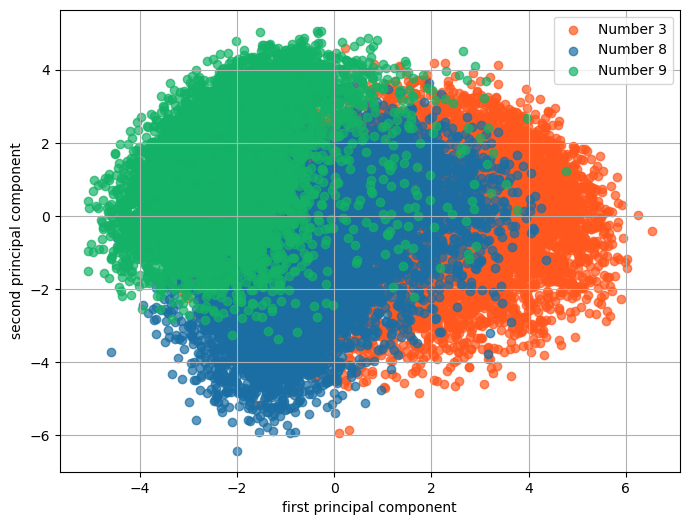
\includegraphics[width=\textwidth]{../img/problem_1/PCA.png}
        \caption{PCA Performance}
        \label{fig:pca}
    \end{subfigure}
    \label{fig:lda_vs_pca}
    \caption{LDA and PCA on MINST dataset}
\end{figure}

\section{Adam and BFGS on Spring Optimization}

\subsection{Convergence Near Optimal Solution}



I implemented the Adam method and BFGS method to optimize the spring system. The final configuration of the spring system is shown in fig.\ref{fig:adam_config} and fig.\ref{fig:bfgs_config}.
\begin{figure}[h!]
    \centering
    % Subfigure for LDA
    \begin{subfigure}[b]{0.45\textwidth}
        \centering
        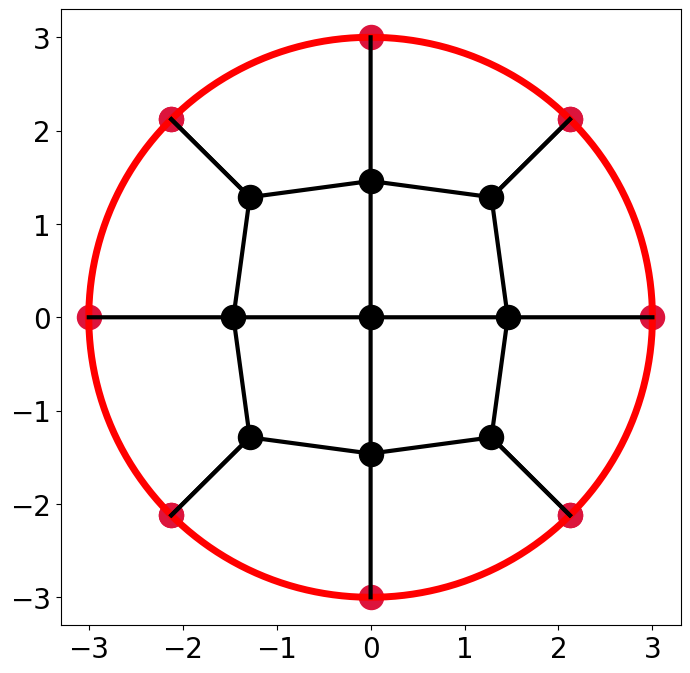
\includegraphics[width=\textwidth]{../img/problem_2/adam.png}
        \caption{Adam final configuration}
        \label{fig:adam_config}
        
    \end{subfigure}
    \hfill
    % Subfigure for PCA
    \begin{subfigure}[b]{0.45\textwidth}
        \centering
        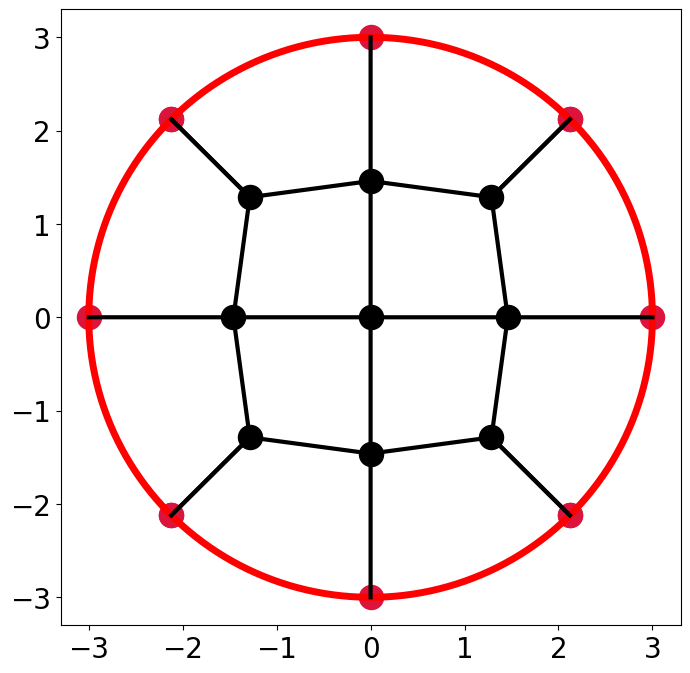
\includegraphics[width=\textwidth]{../img/problem_2/bfgs.png}
        \caption{BFGS final configuration}
        \label{fig:bfgs_config}
    \end{subfigure}
    \label{fig:config}
    \caption{Final Configuration of Spring System Using Adam and BFGS}
\end{figure}

The Adam method converged at:
\[
    \text{iteration}= 187,\quad	\text{energy} = 1.4924514079509037,\quad	\text{gradient norm} = 9.54947425912235\times 10^{-7}
\]
with the final vector:
\begin{align*}
    &\text{theta} = \begin{bmatrix}
        2.35620 & 2.35620 & 3.14160 & 3.92699 \\
        3.92699 & 4.71239 & 5.49779 & 5.49779 \\
        6.28319 & 7.06859 & 7.06859 & 7.85399 \\
    \end{bmatrix}
    \\
    &\text{position} = \begin{bmatrix}
        -1.28645 & -1.33638\times 10^{-5} &  1.28642 & -1.46011 \\
        2.46565\times 10^{-8} &  1.46011 & -1.28642 &  1.33410\times 10^{-5} \\
        1.28645 &  1.28642 &  1.46011 &  1.28645 \\
       -1.33433\times 10^{-5} & -2.12707\times 10^{-8} &  1.33654\times 10^{-5} & -1.28645 \\
       -1.46011 & -1.28642 & & 
    \end{bmatrix}
\end{align*}
while the BFGS method converged at
\[
    \text{iteration}= 31,\quad	\text{energy} = 1.4924514079508941,\quad	\text{gradient norm} = 3.8268520084642785\times 10^{-7}.
\]
whose final vector is almost the same as the Adam method.

\subsection{Performance Near Optimal Solution}

The results are shown in fig.\ref{fig:energy}  and fig.\ref{fig:gradient_norm}. We show that the Adam method decreases linearly when using logarithmic scale, while the BFGS method decreases even faster when the initial position is near the optimal solution.
\begin{figure}[h!]
    \centering
    % Subfigure for LDA
    \begin{subfigure}[b]{0.45\textwidth}
        \centering
        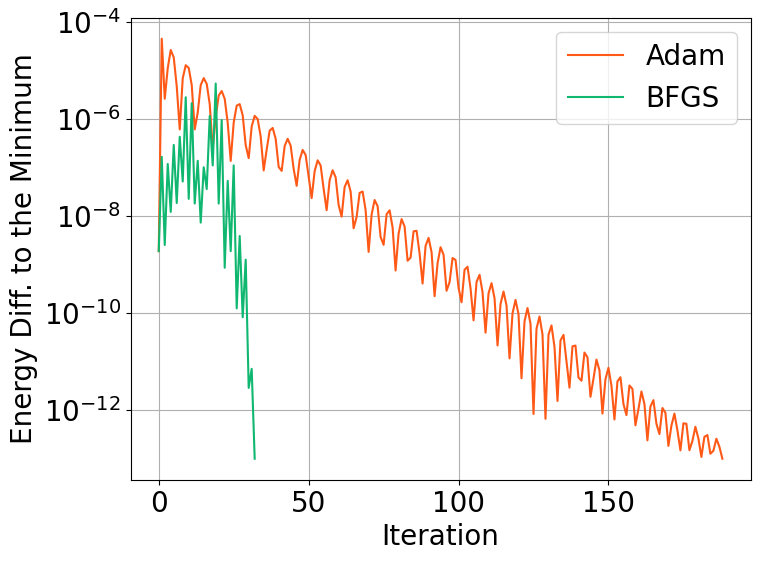
\includegraphics[width=\textwidth]{../img/problem_2/energy.png}
        \caption{Energy vs. Iteration}
        \label{fig:energy}
        
    \end{subfigure}
    \hfill
    % Subfigure for PCA
    \begin{subfigure}[b]{0.45\textwidth}
        \centering
        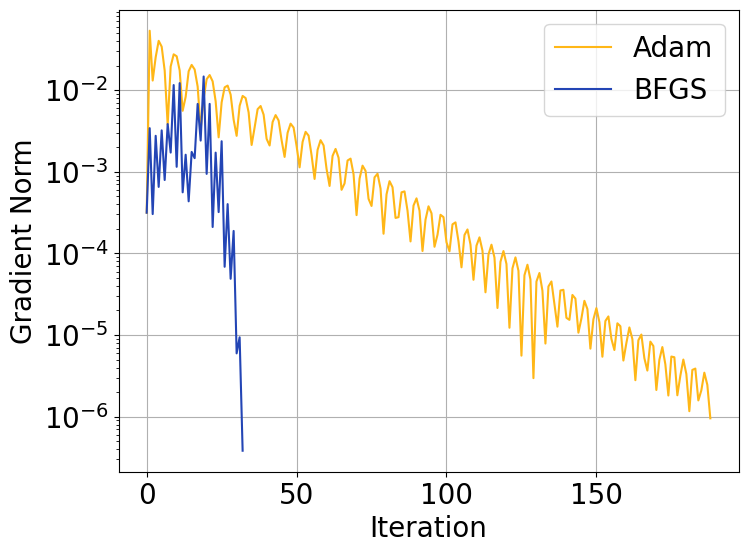
\includegraphics[width=\textwidth]{../img/problem_2/gradient_norm.png}
        \caption{Gradient Norm vs. Iteration}
        \label{fig:gradient_norm}
    \end{subfigure}
    \label{fig:adam_vs_bfgs}
    \caption{Adam and BFGS on Spring Optimization}
\end{figure}

\section{Far from Optimal Solution}

For random generated initial positions, the Adam method fails significantly. The energy and gradient norm are shown in fig.\ref{fig:energy_random} and fig.\ref{fig:gradient_norm_random} in 500 iterations, which is enough for BFGS convergence. 
\begin{figure}[h!]
    \centering
    \begin{subfigure}[b]{0.45\textwidth}
        \centering
        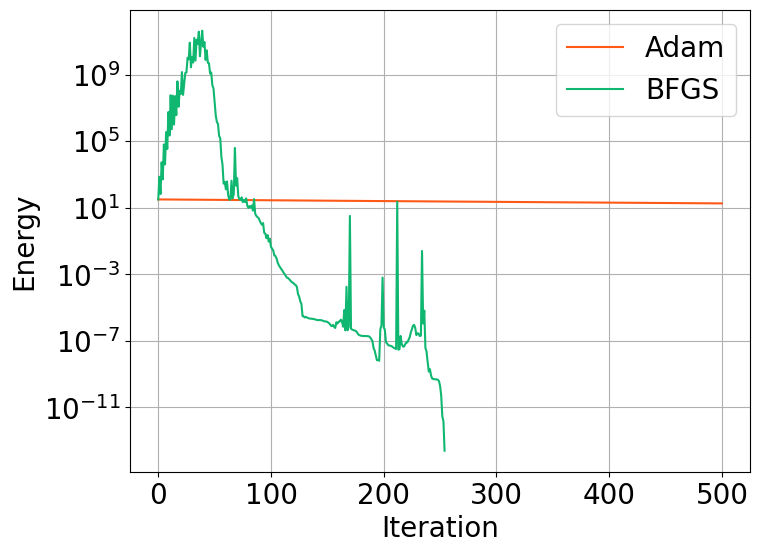
\includegraphics[width=\textwidth]{../img/problem_2/energy_random.png}
        \caption{Energy vs. Iteration}
        \label{fig:energy_random}
        
    \end{subfigure}
    \hfill
    \begin{subfigure}[b]{0.45\textwidth}
        \centering
        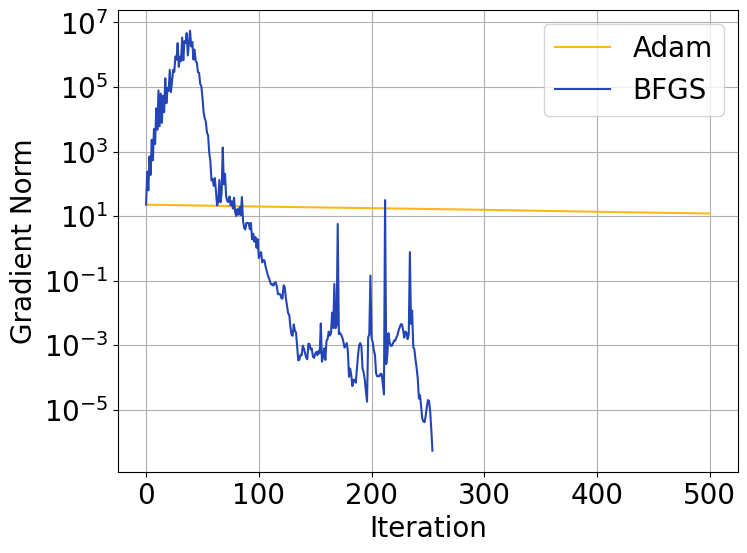
\includegraphics[width=\textwidth]{../img/problem_2/gradient_norm_random.png}
        \caption{Gradient Norm vs. Iteration}
        \label{fig:gradient_norm_random}
    \end{subfigure}
    \label{fig:adam_vs_bfgs_random}
    \caption{Adam and BFGS on Spring Optimization with Random Initial Positions}
\end{figure}

The initial configuration, Adam final configuration and BFGS configuration are shown in fig.\ref{fig:config_random}, fig.\ref{fig:adam_config_random} and fig.\ref{fig:bfgs_config_random} respectively.

\begin{figure}[h!]
    \centering
    % Subfigure for LDA
    \begin{subfigure}[b]{0.3\textwidth}
        \centering
        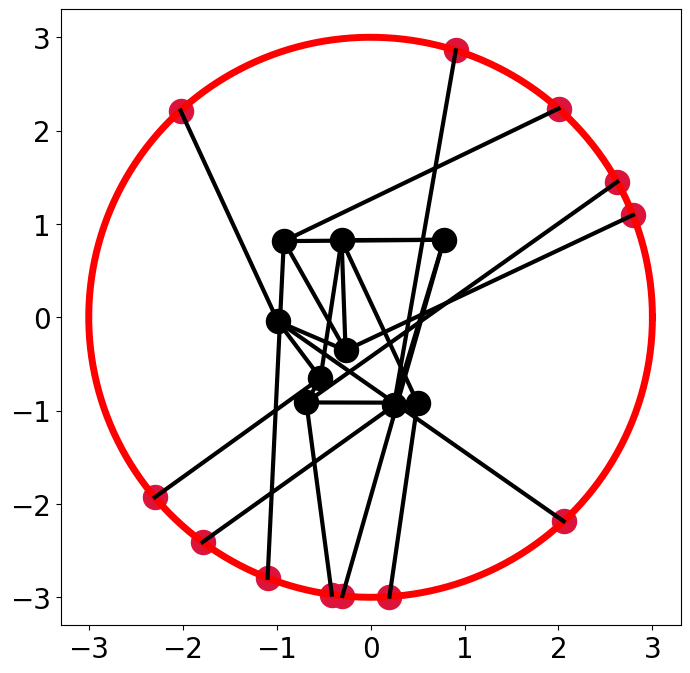
\includegraphics[width=\textwidth]{../img/problem_2/random.png}
        \caption{Initial Configuration}
        \label{fig:config_random}
        
    \end{subfigure}
    \hfill
    % Subfigure for PCA
    \begin{subfigure}[b]{0.3\textwidth}
        \centering
        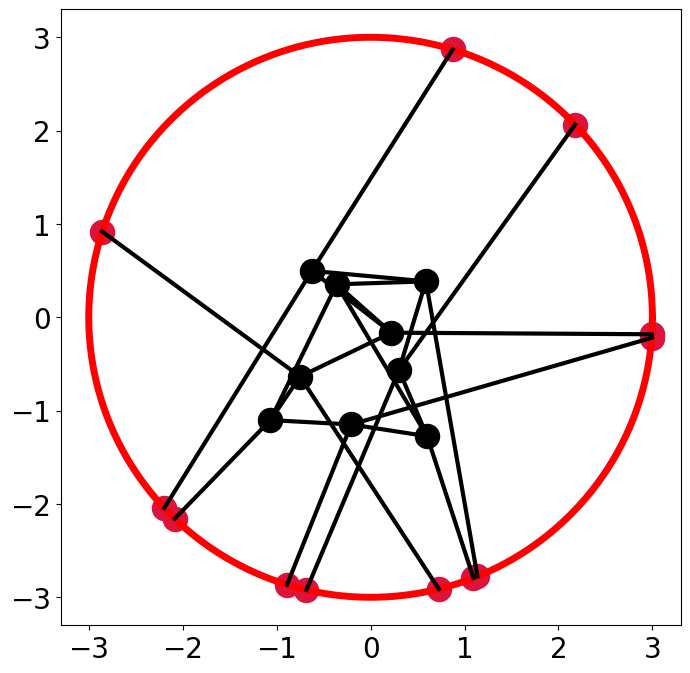
\includegraphics[width=\textwidth]{../img/problem_2/adam_random.png}
        \caption{Adam final configuration}
        \label{fig:adam_config_random}
        
    \end{subfigure}
    \hfill
    % Subfigure for PCA
    \begin{subfigure}[b]{0.3\textwidth}
        \centering
        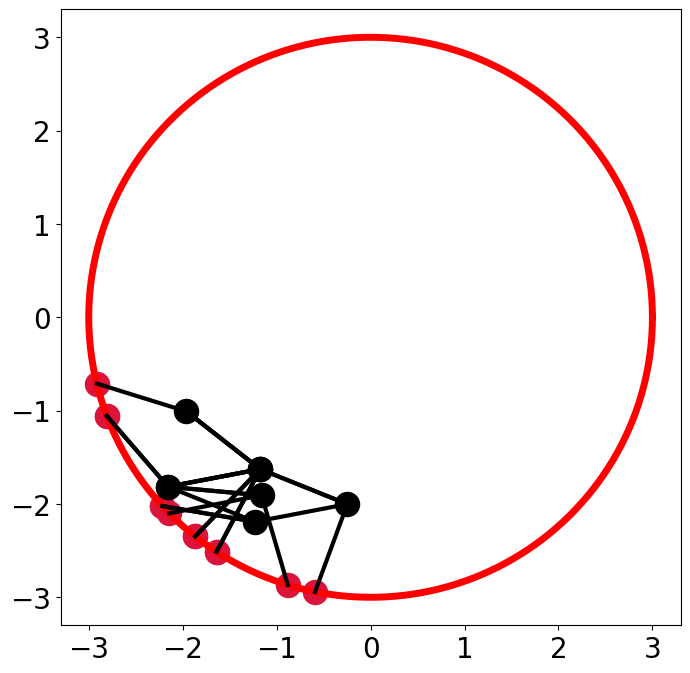
\includegraphics[width=\textwidth]{../img/problem_2/bfgs_random.png}
        \caption{BFGS final configuration}
        \label{fig:bfgs_config_random}
    \end{subfigure}
    \caption{Spring System with Random Initial Positions Using Adam and BFGS}
\end{figure}

\section{Cube \& Sphere Intersection with Monte Carlo}

\subsection{Unit Distribution in a Cube}

Since the volume of the $d$-dimensional unit cube is 1, the fraction of points inside $B^d$ directly gives an estimate of the volume of the intersection of the cube and the sphere. We generate the unit distribution in the cube, which is straightforward by generating $d$ random numbers in $\displaystyle\left[-0.5 ,0.5\right]$ for each dimension. 

Generating $10000000$ points, the results are the following:
\begin{align*}
    & \text{Estimated Vol}(B^5 \cap  C^5) = 0.999568  \\
    & \text{Estimated Vol}(B^{10} \cap C^{10}) = 0.762271  \\
    & \text{Estimated Vol}(B^{15} \cap C^{15}) = 0.197200  \\
    & \text{Estimated Vol}(B^{20} \cap C^{20}) = 0.018337
\end{align*}

\subsection{Unit Distribution in a Ball}

To generate the unit distribution in the ball, we can do it in the following way: first generate a uniform distribution on the unit sphere’s surface, and then generate a radius with the correct volume distribution.

For the frist step, the Gaussian distribution is rotationally symmetric. So normalizing a Gaussian vector gives a uniform direction on the sphere:
\[
    Y=\frac{X}{\|X\|}, \quad X=\left(X_1, X_2, \ldots, X_d\right) \sim \mathcal{N}(0, I)
\]
The second step is to generate the right distribution of its radius from a one-dimension uniform distribution $x\sim u(x), u(x) =1, x\in[0,1]$. Since the cumulative distribution function of the radius $r$ must reflect the volume growth with radius, we have
\[
    F(r) = r^d, \quad r\in[0,1]
\]
As a result:
\begin{align*}
    F'(r) dr = u(x)dx \quad \Rightarrow \quad dx = F'(r)dr \quad \Rightarrow \quad x = r^d
\end{align*}
Therefore, the radius $r$ is generated by $r = x^{1/d}$. The final point is $r\times Y$.

Generating $10000000$ points, the results are the following:
\begin{align*}
    & \text{Estimated Vol}(B^{5} \cap C^5) = 0.997805  \\
    & \text{Estimated Vol}(B^{10} \cap C^{10}) = 0.762488  \\
    & \text{Estimated Vol}(B^{15} \cap C^{15}) = 0.197301  \\
    & \text{Estimated Vol}(B^{20} \cap C^{20}) = 0.018248
\end{align*}


\end{document}
